\documentclass[12pt, letterpaper]{article}
\usepackage[a4paper,left=3cm,right=2cm,top=2.5cm,bottom=2.5cm]{geometry}

\usepackage[utf8]{inputenc}
\usepackage{graphicx}
\graphicspath{ {images/} }
\usepackage{amsmath,bm}
\usepackage{listings}
\usepackage{float}
\usepackage{pdfpages}
\usepackage{siunitx}
\usepackage{subfig}


\title{4TN4 Assignment 4}
\author{Adam Bujak (400113347)}
\date{February 20, 2022}

\begin{document}

\maketitle

\section{Theory}

\subsection{Morphology Operations}

\textbf{Consider the following binary image.}

\begin{table}[!ht]
    \centering
    \begin{tabular}{|l|l|l|l|l|l|l|l|l|l|l|l|}
    \hline
        0 & 0 & 0 & 0 & 0 & 0 & 0 & 0 & 0 & 0 & 0 & 0  \\ \hline
        0 & 0 & 0 & 0 & 0 & 0 & 0 & 0 & 0 & 0 & 0 & 0  \\ \hline
        0 & 0 & 0 & 1 & 1 & 1 & 1 & 1 & 1 & 1 & 0 & 0  \\ \hline
        0 & 0 & 0 & 0 & 1 & 1 & 1 & 1 & 1 & 1 & 0 & 0  \\ \hline
        0 & 0 & 0 & 0 & 0 & 1 & 1 & 1 & 1 & 1 & 0 & 0  \\ \hline
        0 & 0 & 0 & 0 & 0 & 0 & 1 & 1 & 1 & 1 & 0 & 0  \\ \hline
        0 & 0 & 1 & 0 & 0 & 0 & 0 & 1 & 1 & 1 & 0 & 0  \\ \hline
        0 & 0 & 0 & 1 & 0 & 0 & 0 & 0 & 1 & 1 & 0 & 0  \\ \hline
        0 & 0 & 0 & 0 & 1 & 0 & 0 & 0 & 0 & 1 & 0 & 0  \\ \hline
        0 & 0 & 0 & 0 & 0 & 1 & 0 & 0 & 0 & 0 & 0 & 0  \\ \hline
        0 & 0 & 0 & 0 & 0 & 0 & 0 & 0 & 0 & 0 & 0 & 0  \\ \hline
        0 & 0 & 0 & 0 & 0 & 0 & 0 & 0 & 0 & 0 & 0 & 0 \\ \hline
    \end{tabular}
\end{table}

\subsubsection{Erosion}

Apply erosion on the image using the following structuring element.

\[ SE = \begin{bmatrix}0&1&0\\0&1&1\\0&1&0\\ \end{bmatrix} \]


To apply erosion on the image above, each of the pixels (surrounding the operating pixel) that are indicated as "active" by the structuring element are ANDed together.

For example, consider the calculation for the pixel [3,2] (where [x,y] are counted from 0 and the top left of the image)

If we consider the 9 pixels around the pixel [3,2] we have the following matrix:

\[\begin{bmatrix}0&0&0\\0&1&1\\0&0&1\\ \end{bmatrix} \]

given the structuring element above, we only consider the following pixels (x means it is not considered):

\[\begin{bmatrix}x&0&x\\x&1&1\\x&0&x\\ \end{bmatrix} \]

and when we AND together all of the considered pixels we see that we get 0 (since there exists a 0 in the considered set of pixels).

Doing this for each pixel, we get the following image:

\begin{table}[H]
    \centering
    \begin{tabular}{|l|l|l|l|l|l|l|l|l|l|l|l|}
    \hline
        0&0&0&0&0&0&0&0&0&0&0&0 \\ \hline
        0&0&0&0&0&0&0&0&0&0&0&0 \\ \hline
        0&0&0&0&0&0&0&0&0&0&0&0 \\ \hline
        0&0&0&0&0&1&1&1&1&0&0&0 \\ \hline
        0&0&0&0&0&0&1&1&1&0&0&0 \\ \hline
        0&0&0&0&0&0&0&1&1&0&0&0 \\ \hline
        0&0&0&0&0&0&0&0&1&0&0&0 \\ \hline
        0&0&0&0&0&0&0&0&0&0&0&0 \\ \hline
        0&0&0&0&0&0&0&0&0&0&0&0 \\ \hline
        0&0&0&0&0&0&0&0&0&0&0&0 \\ \hline
        0&0&0&0&0&0&0&0&0&0&0&0 \\ \hline
        0&0&0&0&0&0&0&0&0&0&0&0 \\ \hline
    \end{tabular}
\end{table}

\subsubsection{Dilation}

Apply dilation on the image using the following structuring element.

\[ SE = \begin{bmatrix}1&0&0\\0&1&0\\0&0&1\\ \end{bmatrix} \]

The process for the dilation of an image is the exact same as described above for erosion, except instead of ANDing the pixels together we OR them.

For example, consider the calculation for the pixel [3,2] (where [x,y] are counted from 0 and the top left of the image)

If we consider the 9 pixels around the pixel [3,2] we have the following matrix:

\[\begin{bmatrix}0&0&0\\0&1&1\\0&0&1\\ \end{bmatrix} \]

given the structuring element above, we only consider the following pixels (x means it is not considered):

\[\begin{bmatrix}0&x&x\\x&1&x\\x&x&1\\ \end{bmatrix} \]

and when we OR together all of the considered pixels we see that we get 1 (since there exists a 1 in the considered set of pixels).

Doing this for each pixel, we get the following image:

\begin{table}[H]
    \centering
    \begin{tabular}{|l|l|l|l|l|l|l|l|l|l|l|l|}
    \hline
     0 & 0 & 0 & 0 & 0 & 0 & 0 & 0 & 0 & 0 & 0 & 0 \\ \hline
     0 & 0 & 1 & 1 & 1 & 1 & 1 & 1 & 1 & 0 & 0 & 0 \\ \hline
     0 & 0 & 0 & 1 & 1 & 1 & 1 & 1 & 1 & 1 & 0 & 0 \\ \hline
     0 & 0 & 0 & 0 & 1 & 1 & 1 & 1 & 1 & 1 & 1 & 0 \\ \hline
     0 & 0 & 0 & 0 & 0 & 1 & 1 & 1 & 1 & 1 & 1 & 0 \\ \hline
     0 & 1 & 0 & 0 & 0 & 0 & 1 & 1 & 1 & 1 & 1 & 0 \\ \hline
     0 & 0 & 1 & 0 & 0 & 0 & 0 & 1 & 1 & 1 & 1 & 0 \\ \hline
     0 & 0 & 0 & 1 & 0 & 0 & 0 & 0 & 1 & 1 & 1 & 0 \\ \hline
     0 & 0 & 0 & 0 & 1 & 0 & 0 & 0 & 0 & 1 & 1 & 0 \\ \hline
     0 & 0 & 0 & 0 & 0 & 1 & 0 & 0 & 0 & 0 & 1 & 0 \\ \hline
     0 & 0 & 0 & 0 & 0 & 0 & 1 & 0 & 0 & 0 & 0 & 0 \\ \hline
     0 & 0 & 0 & 0 & 0 & 0 & 0 & 0 & 0 & 0 & 0 & 0 \\ \hline
    \end{tabular}
\end{table}

\subsubsection{Opening}

\[ SE = \begin{bmatrix}1&1&1\\1&1&1\\1&1&1\\ \end{bmatrix} \]

To apply opening on an image we perform erosion followed by dilation on an image.

Applying erosion on the image above using the structuring element specified we get the following image:

\begin{table}[H]
    \centering
    \begin{tabular}{|l|l|l|l|l|l|l|l|l|l|l|l|}
    \hline
     0 & 0 & 0 & 0 & 0 & 0 & 0 & 0 & 0 & 0 & 0 & 0 \\ \hline
     0 & 0 & 0 & 0 & 0 & 0 & 0 & 0 & 0 & 0 & 0 & 0 \\ \hline
     0 & 0 & 0 & 0 & 0 & 0 & 0 & 0 & 0 & 0 & 0 & 0 \\ \hline
     0 & 0 & 0 & 0 & 0 & 0 & 1 & 1 & 1 & 0 & 0 & 0 \\ \hline
     0 & 0 & 0 & 0 & 0 & 0 & 0 & 1 & 1 & 0 & 0 & 0 \\ \hline
     0 & 0 & 0 & 0 & 0 & 0 & 0 & 0 & 1 & 0 & 0 & 0 \\ \hline
     0 & 0 & 0 & 0 & 0 & 0 & 0 & 0 & 0 & 0 & 0 & 0 \\ \hline
     0 & 0 & 0 & 0 & 0 & 0 & 0 & 0 & 0 & 0 & 0 & 0 \\ \hline
     0 & 0 & 0 & 0 & 0 & 0 & 0 & 0 & 0 & 0 & 0 & 0 \\ \hline
     0 & 0 & 0 & 0 & 0 & 0 & 0 & 0 & 0 & 0 & 0 & 0 \\ \hline
     0 & 0 & 0 & 0 & 0 & 0 & 0 & 0 & 0 & 0 & 0 & 0 \\ \hline
     0 & 0 & 0 & 0 & 0 & 0 & 0 & 0 & 0 & 0 & 0 & 0 \\ \hline
    \end{tabular}
\end{table}

and then applying dilation on the resulting image using the structuring element specified leaves us with the following image:



\begin{table}[H]
    \centering
    \begin{tabular}{|l|l|l|l|l|l|l|l|l|l|l|l|}
    \hline
     0 & 0 & 0 & 0 & 0 & 0 & 0 & 0 & 0 & 0 & 0 & 0 \\ \hline
     0 & 0 & 0 & 0 & 0 & 0 & 0 & 0 & 0 & 0 & 0 & 0 \\ \hline
     0 & 0 & 0 & 0 & 0 & 1 & 1 & 1 & 1 & 1 & 0 & 0 \\ \hline
     0 & 0 & 0 & 0 & 0 & 1 & 1 & 1 & 1 & 1 & 0 & 0 \\ \hline
     0 & 0 & 0 & 0 & 0 & 1 & 1 & 1 & 1 & 1 & 0 & 0 \\ \hline
     0 & 0 & 0 & 0 & 0 & 0 & 1 & 1 & 1 & 1 & 0 & 0 \\ \hline
     0 & 0 & 0 & 0 & 0 & 0 & 0 & 1 & 1 & 1 & 0 & 0 \\ \hline
     0 & 0 & 0 & 0 & 0 & 0 & 0 & 0 & 0 & 0 & 0 & 0 \\ \hline
     0 & 0 & 0 & 0 & 0 & 0 & 0 & 0 & 0 & 0 & 0 & 0 \\ \hline
     0 & 0 & 0 & 0 & 0 & 0 & 0 & 0 & 0 & 0 & 0 & 0 \\ \hline
     0 & 0 & 0 & 0 & 0 & 0 & 0 & 0 & 0 & 0 & 0 & 0 \\ \hline
     0 & 0 & 0 & 0 & 0 & 0 & 0 & 0 & 0 & 0 & 0 & 0 \\ \hline
    \end{tabular}
\end{table}

\subsection{Distance and Boundary}

\subsubsection{Boundary}
\begin{figure}[H]
    \centering
    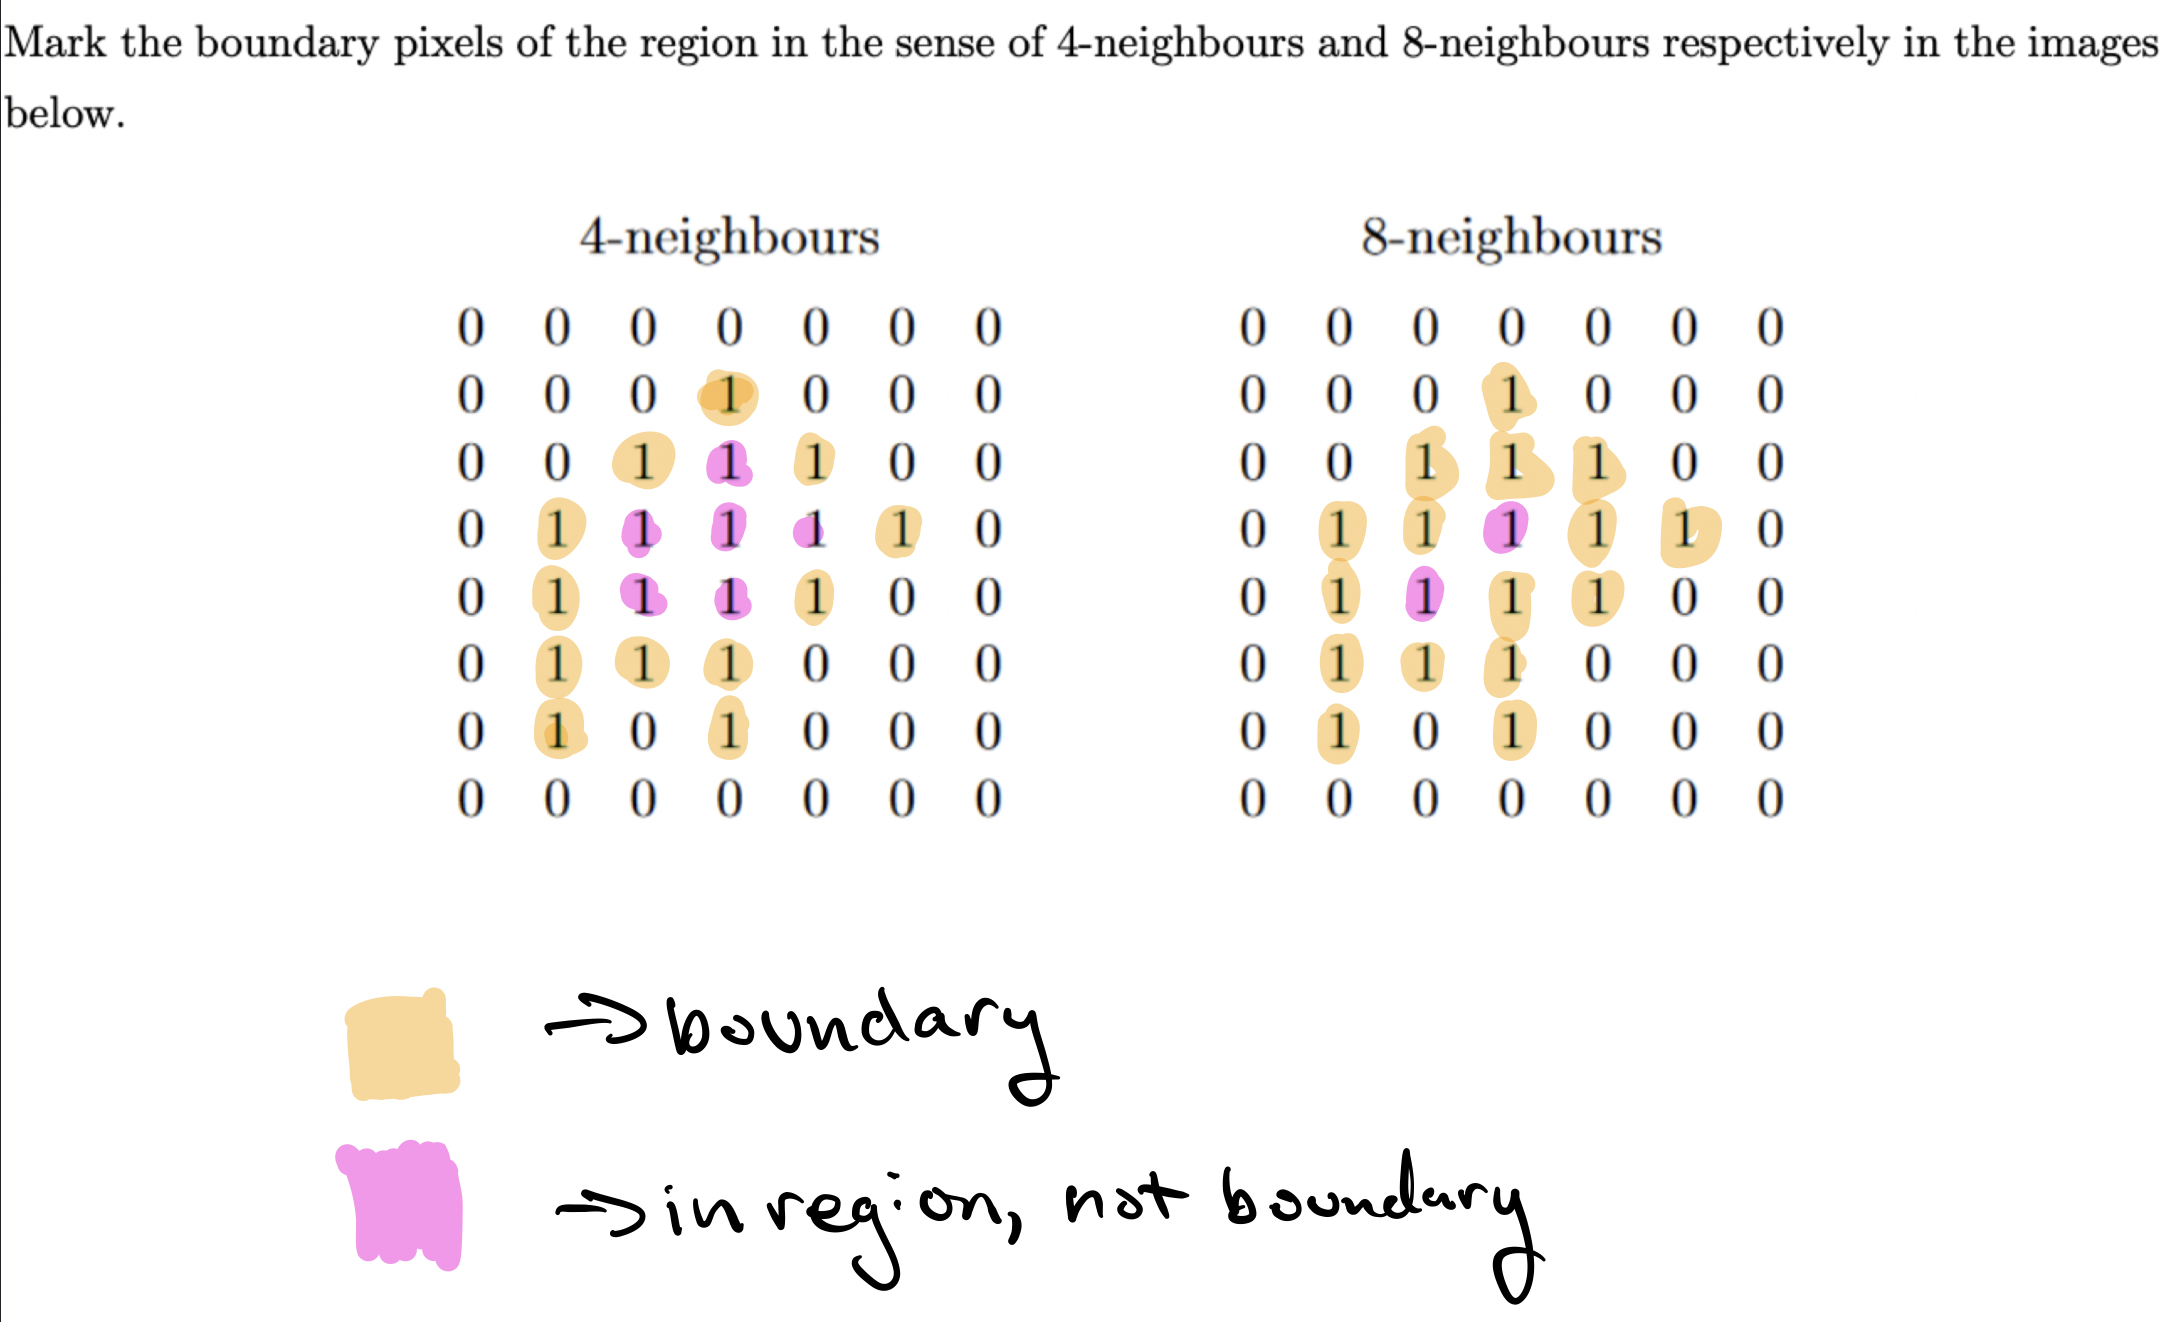
\includegraphics[width=\textwidth]{2.1.png}
\end{figure}

\subsubsection{Distance}


\begin{figure}[H]
    \centering
    \subfloat[\centering 4-neighbors boundary image]{\centering
        \begin{tabular}{|l|l|l|l|l|l|l|}
        \hline
            0 & 0 & 0 & 0 & 0 & 0 & 0 \\ \hline
            0 & 0 & 0 & {\color{red} 1} & 0 & 0 & 0 \\ \hline
            0 & 0 & 1 & 0 & 1 & 0 & 0 \\ \hline
            0 & 1 & 0 & 0 & 0 & 1 & 0 \\ \hline
            0 & 1 & 0 & 0 & 1 & 0 & 0 \\ \hline
            0 & 1 & 1 & 1 & 0 & 0 & 0 \\ \hline
            0 & 1 & 0 & {\color{blue} 1} & 0 & 0 & 0 \\ \hline
            0 & 0 & 0 & 0 & 0 & 0 & 0 \\ \hline
        \end{tabular}}
    \qquad
    \subfloat[\centering 8-neighbors boundary image]{\centering
        \begin{tabular}{|l|l|l|l|l|l|l|}
        \hline
            0 & 0 & 0 & 0 & 0 & 0 & 0 \\ \hline
            0 & 0 & 0 & {\color{red} 1} & 0 & 0 & 0 \\ \hline
            0 & 0 & 1 & 1 & 1 & 0 & 0 \\ \hline
            0 & 1 & 1 & 0 & 1 & 1 & 0 \\ \hline
            0 & 1 & 0 & 1 & 1 & 0 & 0 \\ \hline
            0 & 1 & 1 & 1 & 0 & 0 & 0 \\ \hline
            0 & 1 & 0 & {\color{blue} 1} & 0 & 0 & 0 \\ \hline
            0 & 0 & 0 & 0 & 0 & 0 & 0 \\ \hline
        \end{tabular}}
    \qquad
\end{figure}

\noindent {\textit{NOTE: p is the red pixel, q is the blue pixel} }

\begin{figure}[H]
    \centering
    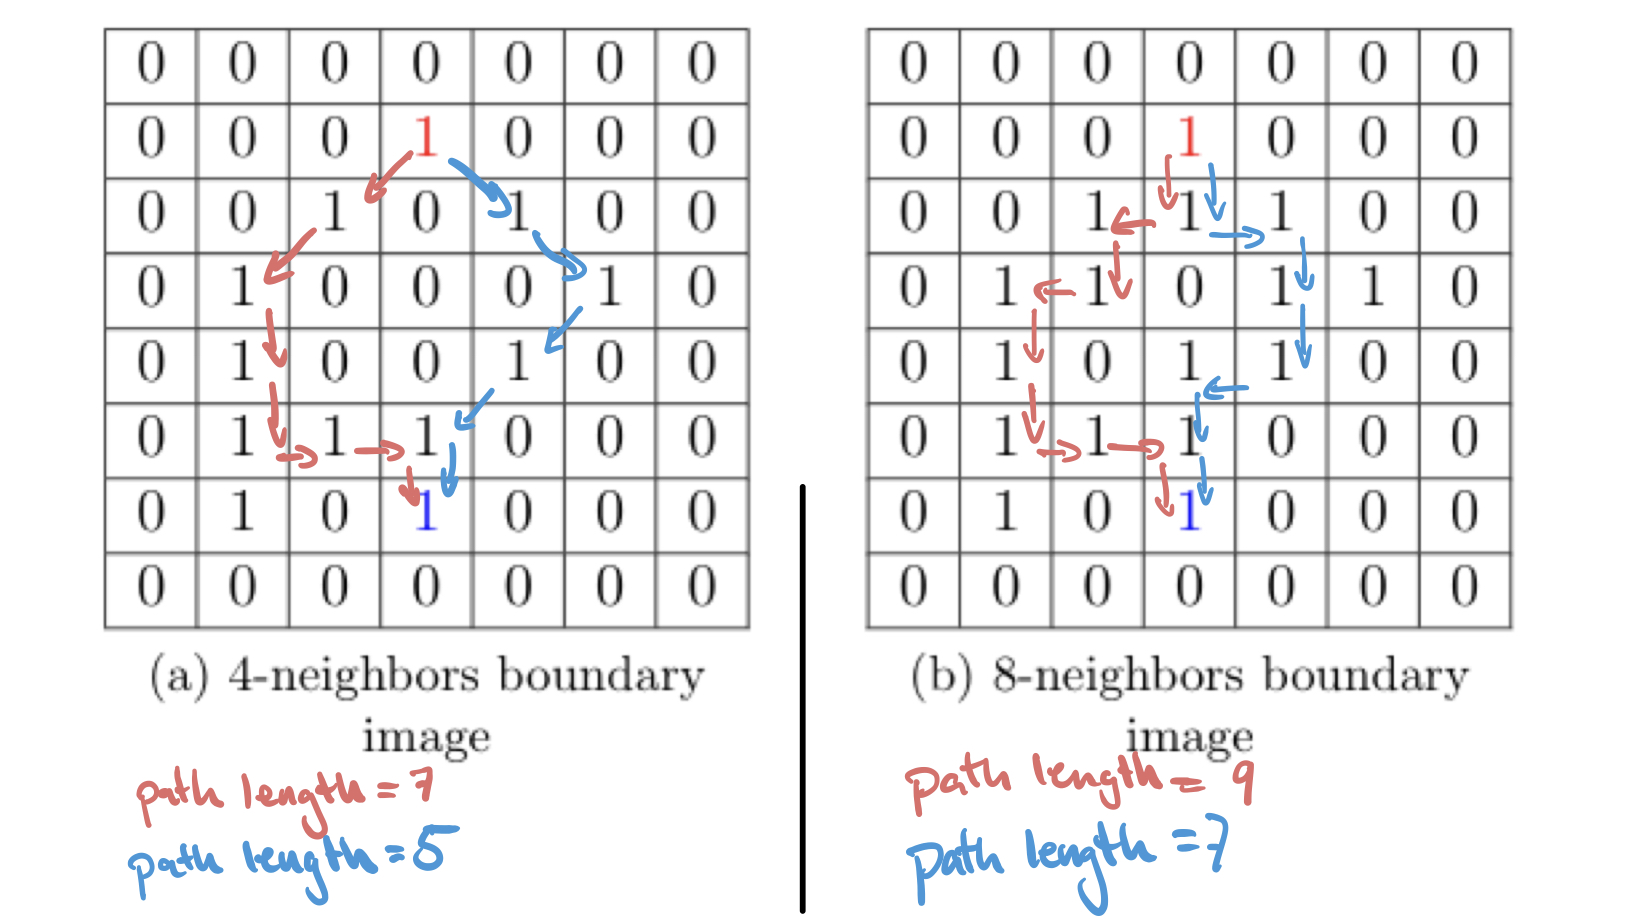
\includegraphics[width=\textwidth]{q2.3.jpeg}
    \caption{$D_m$ distances between p and q in both boundary images}
\end{figure}

\subsubsection{$D_8$ distance of 4-neighbors}

The $D_8$ distance is found by the maximum of the distance in the x direction and the y direction. Thus:

\[ D_8 = max(|x_p-x_q|, |y_p-y_q|) \]

\[ D_8 = max(|3-3|, |1-6|) \]
\[ D_8 = 5 \]

\subsubsection{$D_m$ distance of 4-neighbors}
As shown in Figure 1 a), the $D_m$ distance between p and q is 5.

\subsubsection{$D_m$ distance of 4-neighbors}

The $D_8$ distance is found by the maximum of the distance in the x direction and the y direction. Thus:

\[ D_8 = max(|x_p-x_q|, |y_p-y_q|) \]

\[ D_8 = max(|3-3|, |1-6|) \]
\[ D_8 = 5 \]

\subsubsection{$D_4$ distance of 8-neighbors}

The $D_4$ distance is found by the sum of the distance in the x direction and the y direction. Thus:

\[ D_4 = |x_p-x_q| + |y_p-y_q| \]

\[ D_4 = |3-3| + |1-6| \]
\[ D_4 = 5 \]

\subsubsection{$D_m$ distance of 8-neighbors}
As shown in Figure 1 b), the $D_m$ distance between p and q is 7.

\subsection{Extracting License Plate}

The following is my proposal for an algorithm to detect a license plate in the given image:

\begin{figure}[H]
    \centering
    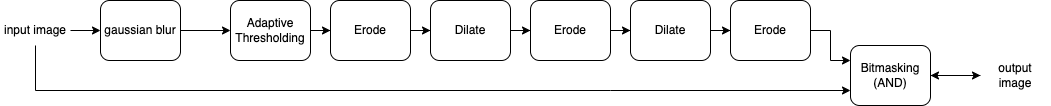
\includegraphics[width=\textwidth]{q3.drawio.png}
\end{figure}

\section{Implementation}

\begin{figure}[H]
    \centering
    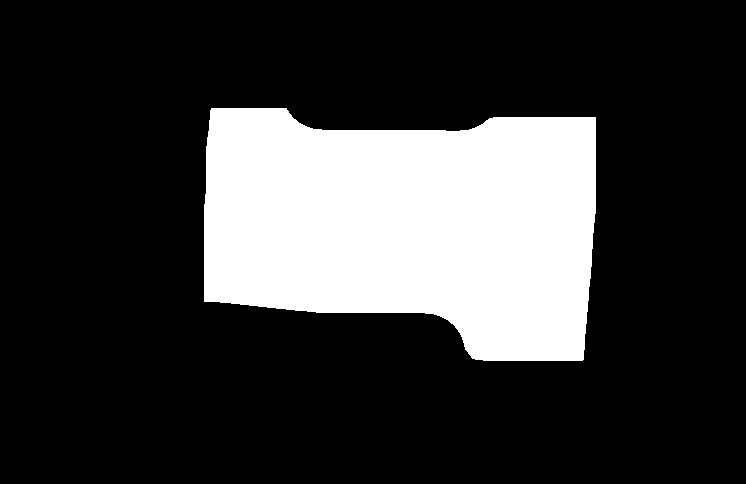
\includegraphics[width=\textwidth]{bitmask.png}
    \caption{Bitmask of where the algorithm thinks the license plate is}
\end{figure}

\begin{figure}[H]
    \centering
    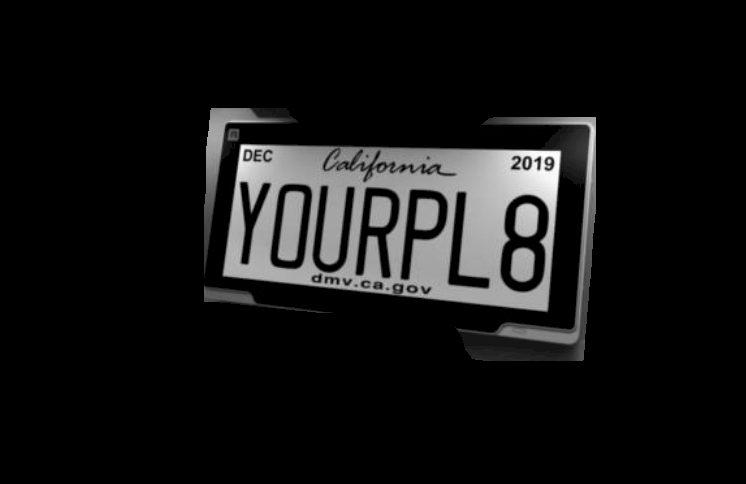
\includegraphics[width=\textwidth]{license.png}
    \caption{Extracted license plate from image}
\end{figure}

\begin{figure}[H]
    \centering
    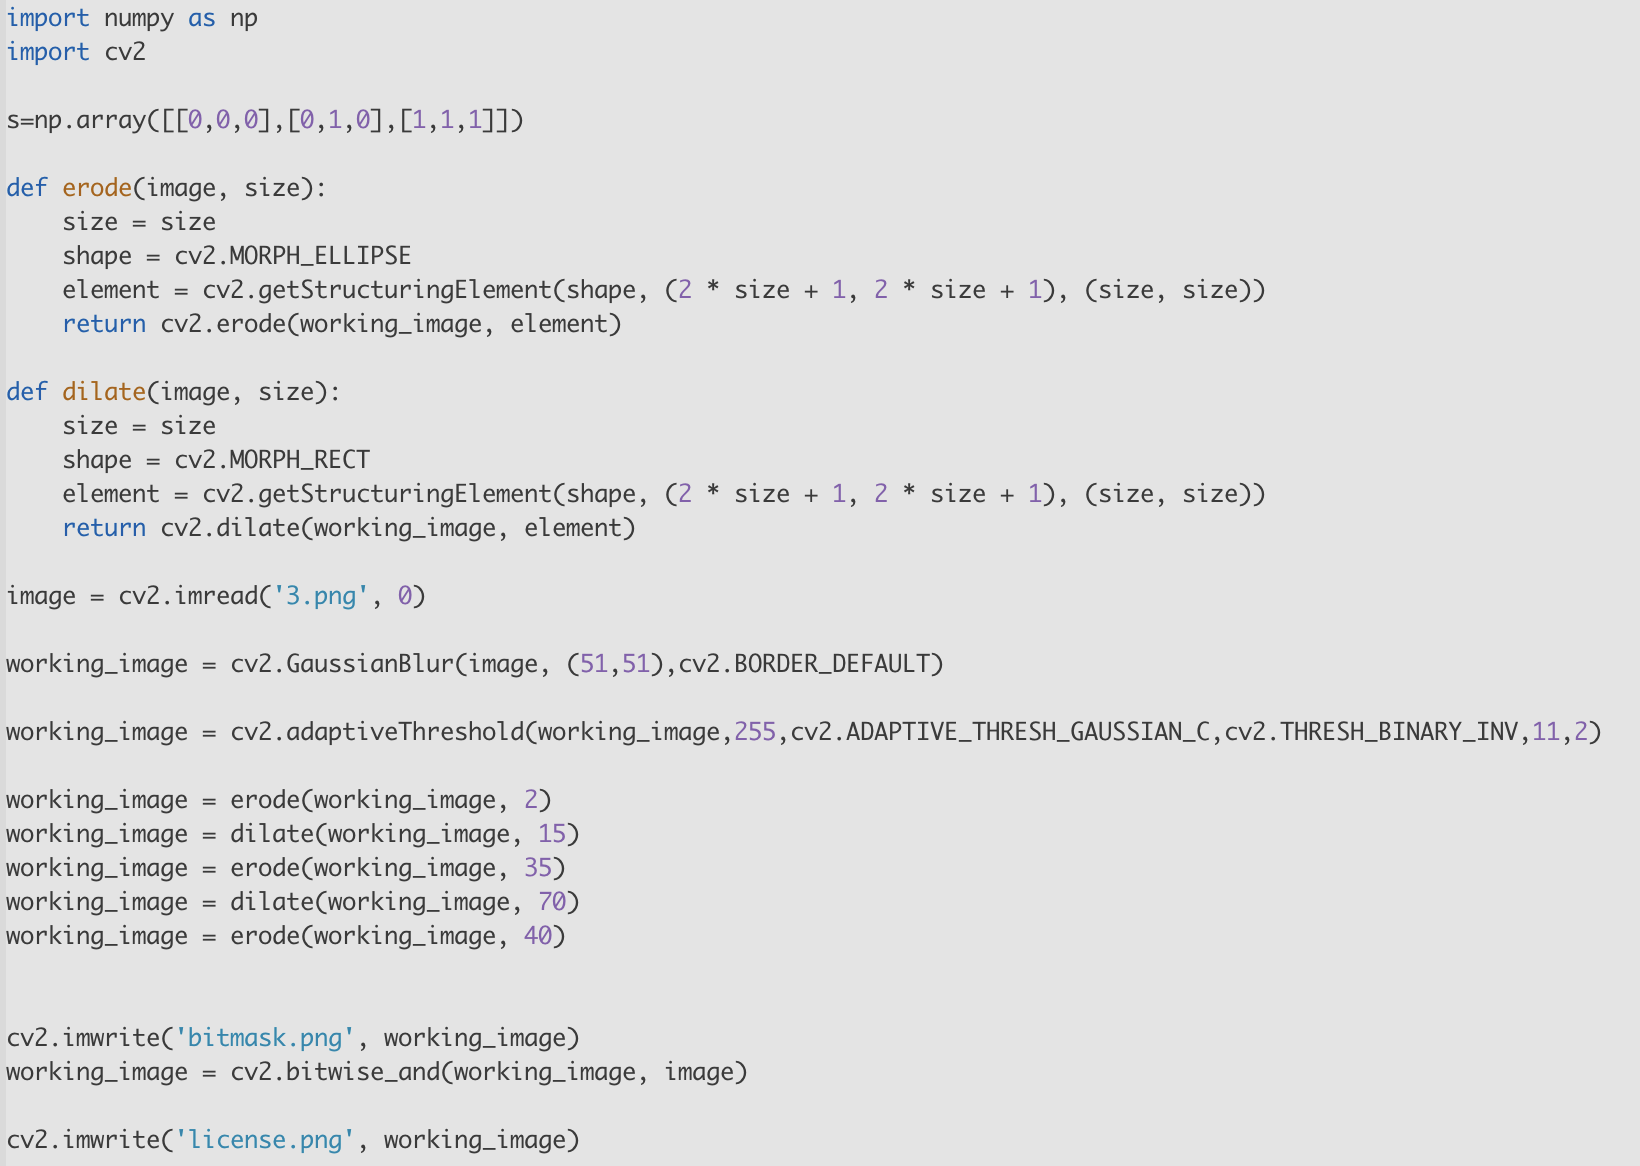
\includegraphics[width=\textwidth]{q3_code.png}
    \caption{Code used to extract license plate}
\end{figure}

The first small erosion removes the lines around the license plate and essentially leaves us with just the letters and a few small artifacts all over the place. Then to preserve the license plate, we dilate heavily, to make all of the letters combine into a blob. Then by eroding to remove the other artifacts, followed by a dilation to merge all the letters once more, and then a final erosion to shrink the blob, we get a bitmask of where the algorithm thinks the license plate is.

This will still work with small changes in angle, scale, and lighting, because it mainly depends on the fact that there are many lines close together in the license plate's text region, which we clump together using dilation, which will remain constant throughout small changes to lighting, angle and scale.

\end{document}

